\chapter{Ondas eletromagnéticas}
\textsl{{\sffamily(Versão: \today)}}

\noindent
Começamos agora o estudo da luz propriamente dita, descrevendo-a como uma
perturbação autoinduzida dos campos elétricos e magnéticos no espaço, regida
pelas leis fundamentais do eletromagnetismo, as equações de Maxwell.

\section{Equações de Maxwell}
As quatro equações de Maxwell para os campos elétrico ($\vec E$) e magnético
($\vec B$) são as seguintes:
\begin{align*}
  \div\vec E&=\frac{\rho}{\epsilon_0}&\div\vec B&=0\\
  \rot\vec E&=-\pd{\vec B}{t}&
  \rot\vec B&=\mu_0\vec j+\mu_0\epsilon_0\pd{\vec E}{t}.
\end{align*}
Nestas expressões, $\epsilon_0=\simeq8,8542\times10^{-12}$\,F/m representa a
permitividade elétrica do vácuo, $\mu_0=4\pi\times10^{-7}$\,H/m a permeabilidade
magnética do vácuo, $\rho$ a densidade de carga (carga por unidade de volume)
total em cada ponto e $\vec j$ a densidade de corrente (corrente elétrica por
unidade de área) total em cada ponto.

Interessam-nos particularmente nestes apontamentos campos variáveis em locais
afastados de cargas e correntes (que constituem, veremos, ondas eletromagnéticas
afastadas das suas fontes). Por isso vamos considerar, para já pelo menos, a
densidade de carga $\rho$ e a densidade de corrente $\vec j$ ambas nulas. As
equações de Maxwell assumem então a forma, mais simétrica, que iremos, quase
sempre, considerar nesta disciplina,\footnote{Para falicitar a referência,
  ordenamos aqui estas equações em ordem crescente da esquerda para a direita e
  de cima para baixo. Assim, chamremos ``primeira equação de Maxwell'' à que
  apresenta a divergência do campo elétrico (lei de Gauss), ``terceira equação
  de Maxwell'' à que envolve o rotacional do mesmo campo (lei de Faraday), etc.}
\begin{equation}\label{eq:meqs}
  \begin{aligned}
    \div\vec E&=0& \div\vec B&=0\\
    \rot\vec E&=-\pd{\vec B}{t}& \qquad\qquad
      \rot\vec B&=\mu_0\epsilon_0\pd{\vec E}{t}.
  \end{aligned}
\end{equation}

Procuremos soluções destas equações. A mais simples de todas é a trivial:
\begin{align*}
  \vec E&=0&\vec B=0.
\end{align*}
É pouco interessante, convenhamos. A seguir, em ordem crescente de complexidade,
consideremos um campo eletromagnético constante e uniforme, isto um campo
elétrico que tem em todos os pontos a mesma intensidade e orientação e que
mantêm essas características inalteradas em todos os instantes, e o mesmo para o
campo magnético. Estes campos têm derivadas todas nulas em todos os pontos e em
todos os instantes e, assim, são também solução das equações de Maxwell. Mas há
uma certa quantidade de energia associada ao campo, e um campo uniforme (ou
seja, definido em todo o espaço com uma mesma intensidade e orientação) tem uma
energia infinita. São, assim, soluções não realistas das equações de
Maxwell e por isso não a consideraremos (excepto se $\vec E$ e $\vec B$ forem
constante e uniformemente nulos, caso que já tratámos). Resumindo:

Consideremos agora o caso dos campos que dependem de ponto para ponto, mas são
constantes (independentes do tempo). Suponhamos, por exemplo, que o campo
magnético $\vec B$ é constante, mas apresenta valores e/ou orientações
diferentes de ponto para ponto. Então $\partial \vec B/\partial t=0$; a terceira
equação de Maxwell mostra então que $\rot \vec E=0$. Mas um campo com
divergência nula e com rotacional nulo é um campo com todas as derivadas
espaciais nulas, ou seja, um campo uniforme. Concluímos que $\vec E$ é uniforme
e, pelas razões atrás apresentadas, só pode ser nulo em todo o espaço,
constantemente nulo, entenda-se. Então a derivada $\partial \vec E/\partial t$
anula-se; logo, de acordo com a última das equações, $\rot \vec B=0$: o campo
magnético, afinal, tem as derivadas espaciais todas nulas! Logo, é uniforme e,
portanto, como vimos no parágrafo anterior, só pode ser nulo.

\section{Ondas eletromagnéticas}
Verificámos que campos uniformes e constantes só podem ser nulos, que campos
constantes (mesmo que não sejam uniformes) também só podem ser nulos, e
poderíamos verificar (tente fazê\-\mbox{-lo}!) que campos uniformes (mesmo que não sejam
constantes) também devem anular-se. Ou seja, que soluções constantes e/ou
uniformes constituem, na realidade, a solução trivial $\vec E=\vec B=0$.
Vamos agora considerar situações mais interessantes, em que os campos dependem da
posição \emph{e} do tempo.

\subsection*{Um caso particular ilustrativo}
Mantendo a situação o mais simples possível, consideremos um campo elétrico que
depende do tempo e de apenas uma coordenada espacial, que escolhemos ser a
coordenada $x$,
\begin{equation*}
  \vec E=\vec E(x,t).
\end{equation*}
Como o campo (as três componentes do campo) só dependem de $t$ e de $x$, as suas
derivadas relativamente às outras coordenadas $y$ e $z$ são nulas, isto é,
\begin{align*}
  \pd{\vec E}{y}=\pd{\vec E}{z}=0,
\end{align*}
e repare que afirmar que as derivadas do vetor campo elétrico se anulam
significa dizer que se anulam as derivadas \emph{de cada componente} do campo
elétrico.

Tendo em conta a expressão da divergência de um campo vetorial da
\eqref{eq:divcart}, a primeira das equações de Mawell pode também escrever-se
como
\begin{equation*}
  \pd{E_x}{x}+\pd{E_y}{y}+\pd{E_z}{z}=0,
\end{equation*}
que, de acordo com o que acabámos de discutir, se reduz neste caso em que o
campo só depende da coordenada $x$ a
\begin{equation*}
  \pd{E_x}{x}=0,
\end{equation*}
ou seja, a componente $x$ do campo é uniforme. Mas então, como vimos na secção
anterior, deve ser nula, $E_x=0$. Estes argumentos podem ser aplicados sem
alteração para o campo magnético, ou considerando campos que dependem apenas da
coordenada $y$ ou $z$. Podemos assim concluir que se o campo elétrico ou o campo
magnético dependem apenas de uma das coordenadas, então a componente
correspondente a essa coordenada é nula.

Dado que $E_x=0$ e que $\partial E_\alpha/\partial y=\partial E_\alpha/\partial
z=0$ (qualquer que seja a componente $E_\alpha$ do campo), as equações para o
rotacional dos campos elétrico e magnético (na segunda linha das
eqs.~\eqref{eq:meqs}), tendo em conta a expressão do rotacional em coordenadas
cartesianas da eq.~\eqref{eq:rotcart}, podem escrever-se como
\begin{subequations}
\begin{align}
  0&=-\pd{B_x}{t}&        \pd{B_z}{y}-\pd{B_y}z&=0\label{eq:meqx}\\
  \pd{E_z}{x}&=\pd{B_y}{t}&  \pd{B_x}{z}-\pd{B_z}{x}&=
    \epsilon_0\mu_0\pd{E_y}{t} \label{eq:meqy}\\
  \pd{E_y}{x}&=-\pd{B_z}{t}& 
    \pd{B_y}{x}-\pd{B_y}{x}&=\epsilon_0\mu_0\pd{E_z}{t}\label{eq:meqz}
\end{align}
\end{subequations}
Tomemos a igualdade no lado esquerdo da eq.~\eqref{eq:meqy} e derivêmo-la em
ordem a $x$. Resulta
\begin{equation*}
  \pdd{E_z}{x}=\pd{}{t}\pd{B_y}{x}.
\end{equation*}
Mas a igualdade no lado direito da eq.~\eqref{eq:meqy} pode escrever-se como
\begin{equation*}
  \pd{B_y}{x}=\pd{B_y}{x}+\epsilon_0\mu_0\pd{E_z}{t}.
\end{equation*}
Substituindo em cima, obtemos
\begin{equation*}
  \pdd{E_z}{x}=\pd{}{t}\pd{B_y}{x}+\epsilon_0\mu_0\pdd{E_z}{t}
\end{equation*}
O primeiro termo no lado direito desta igualdade é nulo:
\begin{equation*}
  \pd{}{t}\pd{B_y}{x}=\pd{}{x}\pd{B_y}{t}=0,
\end{equation*}
de acordo com a equação no lado esquerdo da primeira linha. Obtemos então, por
fim,
\begin{equation*}
  \pdd{E_z}{x}=\epsilon_0\mu_0\pdd{E_z}{t}.
\end{equation*}
Mas repare-se que esta é a equação diferencial satisfeita em geral por ondas que
se propagam ao longo do eixo dos $x$ sem alteração de forma (veja a
eq.~\eqref{eq:waveq}), com velocidade
$v=1/\sqrt{\mu_0\epsilon_0}=3,00\times10^{8}$\,m/s.  Verificamos assim que as
equações de Maxwell admitem soluções que representam ondas que se propagam sem
alteração de forma com a velocidade da luz. Nesta análise, constatámos também que a
componente $x$ do campo elétrico é nula. Mas a direção do eixo dos $x$ é a
direção de propagação.  Assim, constatamos que o campo elétrico, neste exemplo,
é transversal. Veremos que se trata de uma propriedade geral do campo elétrico
(e também do magnético) numa onda eletromagnética.

\subsection{Análise mais geral}
Depois de apresentado o exemplo anterior, vejamos isto com maior generalidade.
Calculemos o rotacional da terceira equação de Maxwell, na linha de baixo e à
esquerda na eq.~\eqref{eq:meqs}:
\begin{equation*}
  \rot\rot\vec E=-\rot\pd{\vec B}{t}=-\pd{}{t}\rot\vec B.
\end{equation*}
Mas o rotacional do campo magnético é dado pela quarta equação de Maxwell.
Substibuindo aqui, obtemos
\begin{equation*}
  \rot\rot\vec E=-\epsilon_0\mu_0\pdd{\vec E}{t}.
\end{equation*}
O rotacional duplo do lado esquerdo desta igualdade pode simplificar-se
aplicando um teorema da análise de funções de várias variáveis segundo o qual
para qualquer função vetorial $\vec A$ se tem
\begin{equation*}
  \rot\rot\vec A=\grad\div\vec A - \lap\vec A.
\end{equation*}
No caso que estudamos, o primeiro termo é nulo porque, de acordo com a primeira
equação de Maxwell, $\div \vec E=0$. Resulta então, por fim,
\begin{equation}\label{eq:efplw}
  \lap\vec E=\epsilon_0\mu_0\pdd{\vec E}{t}.
\end{equation}
Mas esta é a equação geral das ondas planas em três dimensões, que deduzimos no
capítulo anterior (veja a eq.~\eqref{eq:plweq3d}). Concluímos assim, com toda a
generalidade que o campo elétrico pode existir no vazio em configurações não
triviais, na forma de ondas planas que se propagam à velocidade da luz
$c=1/\sqrt{\epsilon_0\mu_0}$ sem alteração de forma.

Poderíamos ter começado por calcular o rotacional da quarta equação de Maxwell.
Chegaríamos a uma equação semelhante à eq.~\eqref{eq:efplw} mas envolvendo agora
o campo magnético.

Agora que sabemos que há soluções das equações de Maxwell que satisfazem a
equação de onda, podemos descrever o campo elétrico (e o campo magnético também) 
com as fuções de onda harmónicas, que já vimos serem soluções da dita equação de
onda. Assim, seja o campo elétrico dado por
\begin{equation}\label{eq:hpwef}
  \vec E(\vec r,t)=\vec E_0\,\e^{\iu(\vec k\cdot\vec r-\omega t+\phi_0)}.
\end{equation}
Nesta expressão, os símbolos $\vec k$, $\omega$ e $\phi_0$ têm o significado que
já lhes atribuímos no capítulo anterior\footnote{$\vec k$ é o vetor de onda, com
  a direção e o sentido da propagação e com módulo $k=2\pi/\lambda$,
$\omega=2\pi/T$ é a frequência angular da onda e $\phi_0$ é a constante de
fase.}, mas na amplitude amplitude ($\vec E_0$) talvez se estranhe o caráter
vetorial explicitado pela setinha. Bem, como discutimos no primeiro capítulo, a
amplitude de uma onda harmónica tem a natureza da função de onda, tanto quanto
às dimensões e unidades, como quanto ao caráter escalar/vetorial. Como a função
de onda é o campo elétrico e como este é um vetor, a amplitude desta onda
harmónica é igualmente um vetor. Chama-se \emph{direção de polarização} da onda
à direção do vetor amplitude dessa onda.

Vamos agora estudar as propriedades desta onda de campo elétrico, analisando-a à
luz das equações de Maxwell. Antes, porém, vejamos como atuam os operadores
diferenciais numa função de onda como a da eq.~\eqref{eq:hpwef}. Ao mesmo tempo
que facilitará a análise que vamos fazer a seguir, este estudo revelará as
vantagens da forma exponencial complexa sobre as formas trignométricas.

Note que a expressão $\vec k\cdot\vec r$ é o produto escalar do vetor de onda
$\vec k$, com componentes $(k_x,\,k_y,\,k_z)$ e do vetor posição
$\vec r=(x,\,y,\,z)$. Assim, $\vec k\cdot\vec r=k_xx+k_yy+k_zz$;
logo,
\begin{align*}
  \pd{}{x}\e^{\iu(\vec k\cdot\vec r-\omega t+\phi_0)}&=
  \iu k_x\e^{\iu(\vec k\cdot\vec r-\omega t+\phi_0)}
\end{align*}
e, do mesmo modo,
\begin{align*}
  \pd{}{y}\e^{\iu(\vec k\cdot\vec r-\omega t+\phi_0)}&=
  \iu k_y\e^{\iu(\vec k\cdot\vec r-\omega t+\phi_0)}&
  \pd{}{z}\e^{\iu(\vec k\cdot\vec r-\omega t+\phi_0)}&=
  \iu k_z\e^{\iu(\vec k\cdot\vec r-\omega t+\phi_0)}
\end{align*}
As derivadas do campo elétrico da eq.~\eqref{eq:hpwef} são, então, dadas por
expressões simples. Por exemplo, a derivada em ordem a $x$ fica
\begin{equation*}
  \pd{}{x}\vec E=\vec E_0\pd{}{x}\e^{\iu(\vec k\cdot\vec r-\omega t+\phi_0)}=
  \iu k_x\vec E_0\e^{\iu(\vec k\cdot\vec r-\omega t+\phi_0)}=
  \iu k_x \vec E.
\end{equation*}
Expressões semelhantes obtêm-se para as restantes derivadas. Em resumo,
\begin{align*}
  \pd{\vec E}{x}&=\iu k_x\vec E&
  \pd{\vec E}{y}&=\iu k_y\vec E&
  \pd{\vec E}{z}&=\iu k_z\vec E&
  \pd{\vec E}{t}&=-\iu \omega\vec E.
\end{align*}
Essencialmente, é a simplicidade destas expressões que torna a representação das
funções harmónicas com exponenciais complexas vantajosa. Se mantivessemos a
representação com funções trignométricas, o cálculo das derivadas parciais da
função de onda seria muito mais complexo\footnote{Mas é um bom exercício
fazê-lo.  Força!}.

\subsection{As ondas eletromagnéticas são ondas transversais}
De acordo com a primeira equação de Maxwell, a divergência do campo elétrico é
nula. Mas, dada a expressão geral da divergência em coordenadas cartesianas 
(eq.~\eqref{eq:divcart}) e as igualdades que acabámos de demonstrar, temos
\begin{align*}
  \div\vec E&=\pd{E_x}{x}+\pd{E_y}{y}+\pd{E_z}{z}\\
            &=\iu k_x E_x+\iu k_y E_y+\iu k_z E_z=\iu\vec k\cdot\vec E.
\end{align*}
Se a divergência do campo é nula, é nulo o produto escalar do campo com o vetor
de onda $\vec k$. Logo, o campo elétrico é perpendicular ao vetor de onda, ou
seja, é perpendicular à direção de propagação.

Consideremos agora a terceira equação de Maxwell:
\begin{align*}
  \pd{\vec B}{t}&=-\rot\vec E\\
                &=-\rot \vec E_0\e^{\iu(\vec k\cdot\vec r-\omega t+\phi_0)}
  =-\vec \nabla\times\vec E_0\e^{\iu(\vec k\cdot\vec r-\omega t+\phi_0)}\\
  &=-\iu\vec k\times\vec E_0\e^{\iu(\vec k\cdot\vec r-\omega t+\phi_0)}.
\end{align*}
Então o campo magnético pode obter-se primitivando em ordem ao tempo o lado
direito, ou seja,
\begin{align}
  \vec B&=-\iu\vec k\times\vec E_0\int\e^{\iu(\vec k\cdot\vec r-\omega
          t+\phi_0)}dt\nonumber\\
          &=-\iu\vec k\times\vec E_0\frac{1}{-i\omega}
            \e^{\iu(\vec k\cdot\vec r-\omega t+\phi_0)}\nonumber\\
            \vec B&=\frac{1}{\omega}\vec k\times \vec E.\label{eq:mf}
\end{align}
Vemos assim que o campo magnético associado a uma onda plana eletromagnética é
proporcional ao produto vetorial do vetor de onda com o campo. Ou seja,
é perpendicular ao campo elétrico e também à direção de propagação: numa onda
eletromagnética plana, ambos os campos são transversais, e são perpendiculares
entre si. 

De acordo com a eq.~\eqref{eq:mf}, o campo magnético pode escrever-se como
\begin{equation*}
  \vec B=\vec B_0\,\e^{\iu(\vec k\cdot\vec r-\omega t+\phi_0)},\qquad
  \text{ com } 
  \vec B_0=\frac{1}{\omega}\vec k\times\vec E_0.
\end{equation*}
Este resultado mostra que o campo magnético constitui também uma onda plana
harmónica, com a mesma direção de propagação, a mesma frequência e o mesmo
comprimento que o campo elétrico, e com a mesma fase também. Para além disso, os
módulos das amplitudes do campo magnético e do campo elétrico estão também
relacionados. Uma vez que $\vec E_0$ e $\vec k$ são perpendiculares, o módulo do
produto vetorial é igual ao produto dos módulos dos dois vetores e, assim,
\begin{equation}\label{eq:b0e0}
  B_0 = \frac{k}{\omega}E_0=\frac{E_0}{c},
\end{equation}
onde $c$ representa a velocidade de propagação da onda.

A Figura~\ref{fig:plemwave} ilustra a orientação relativa do campo elétrico, do
campo magnético e da direção de propagação, para uma direção de polarização
coincidente com o eixo dos $y$.
\begin{figure}[htb]
  {\centering
      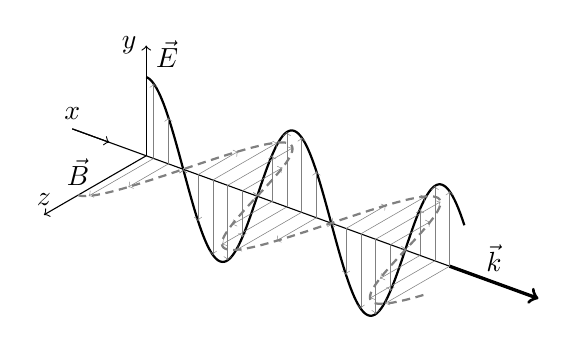
\begin{tikzpicture}[x={(-20:1cm)},y={(90:1cm)},z={(210:1cm)}]
        % Axes
        \draw (-1,0,0) node[above] {$x$} -- (5,0,0);
        \draw [->] (-1,0,0) -- (-0.5,0,0);
        \draw [->](0,0,0) -- (0,1.4,0) node[left] {$y$};
        \draw [->] (0,0,0) -- (0,0,1.5) node[above] {$z$};
        % Propagation
        \draw[->,very thick] (4.1,0,0) -- node[above] {$\vec k$} (5.3,0,0);
        % Waves
        \draw[thick] plot[domain=0:4.3,samples=200] (\x,{cos(deg(pi*\x))},0);
        \draw[gray,thick, densely dashed] plot[domain=0:4.3,samples=200]
        (\x,0,{cos(deg(pi*\x))});
        % Arrows
        \foreach \x in {0.1,0.3,...,4.2} {
          \draw[->,help lines] (\x,0,0) -- (\x,{cos(deg(pi*\x))},0);
          \draw[->,help lines] (\x,0,0) -- (\x,0,{cos(deg(pi*\x))});
        }
        % Labels
        \node[above right] at (0,1,0) {$\vec{E}$};
        \node[above] at (0,0,1) {$\vec{B}$};
      \end{tikzpicture}\par
    }
    \caption{Onda eletromagnética plana e harmónica que se propaga no sentido
    positivo do eixo dos $x$, com direção de polarização (a direção do campo
  elétrico) segundo o eixo dos $y$ e campo magnético paralelo ao eixo dos $z$.
  (Adaptado de um artigo no \LaTeX{} StackExchange.)\label{fig:plemwave}}
\end{figure}

\section{O vetor de Poynting e a irradiância}
O campo elétromagnético armazena e transporta energia. Isto é, é necessário
dispender energia para criar os campos elétrico e/ou magnético definidos numa
região do espaço e esses campos podem transportar energia para outras regiões do
espaço. 

O transporte de energia pelo campo é completamente caracterizado pelo
\emph{vetor de Poynting,}
\begin{equation}
  \vec S=\frac{1}{\mu_0}\vec E\times\vec B.
\end{equation}
A orientação deste vetor é a do fluxo de energia; o seu módulo é a quantidade de
energia transportada por unidade de tempo e de área perpendicular a esse fluxo.

Numa onda de luz, o módulo do vetor de Poynting oscila com frequência muito
elevada, e por isso é mais informativo tomar médias temporais. A
\emph{irradiância} (ou \emph{densidade de fluxo radiante}) é uma destas médias.
Define-se como a potência (energia por unidade de tempo) transferida por unidade
de área e é o valor médio do módulo do vetor de Poynting ao longo de um período
da sua oscilação.

Numa onda harmónica plana como as que estudámos na secção anterior, os dois
campos $\vec E$ e $\vec B$ são perpendiculares. Assim, o módulo do vetor de
Poynting é dado por
\begin{align*}
  S&=\|\vec S\|=\frac{1}{\mu_0}EB=
  \frac{E_0B_0}{\mu_0}\cos^2\left(\vec k\cdot\vec r-\omega t+\phi_0\right)\\
  &=
  \frac{E^2_0}{\mu_0c}\cos^2\left(\vec k\cdot\vec r-\omega t+\phi_0\right),
\end{align*}
onde $E_0$ e $B_0$ representam respetivamente os módulos das amplitudes dos
campos elétrico e magnético e se usou a igualdade~\eqref{eq:b0e0}. Note-se que
não podemos aqui usar a representação complexa, porque a expressão envolve um
produto de duas funções trignométricas; ocorre aqui, por isso, a ``infeção'' da
parte real da representação (com significado físico) pela sua parte imaginária
(aqui irrelevante) que foi referida na secção secção~\ref{sec:complexharm}.  O
valor médio desta função calculado ao longo de um período é
\begin{equation*}
  I=\overline S=\frac{1}{T}\int_{0}^TS(t)dt=\frac{E_0^2}{\mu_0cT}
  \int_0^T\cos^2\left(\vec k\cdot\vec r-\omega t+\phi_0\right)dt.
\end{equation*}
Mas $\cos^2\theta=(1+\cos2\theta)/2$; então,
\begin{equation*}
  I=\frac{E_0^2}{2\mu_0cT}
  \int_0^T\left[1+\cos2\left(\vec k\cdot\vec r-\omega t+\phi_0\right)\right]dt.
\end{equation*}
O integral da primeira parcela é, simplesmente, $T$; o segundo, sendo o integral
da função cosseno ao longo de um período completo, anula-se. Então, resulta por
fim
\begin{equation}
  I=\frac{E_0^2}{2\mu_0c}=\frac{1}{2}\epsilon_0cE_0^2.
\end{equation}


\section{Polarização}
\tobedone{}

\section{O espetro eletromagnético}
A luz é então uma onda eletromagnética. Mas nem todas as ondas eletromagnéticas
são luz (visível). Os nosso sistema visual (olhos e cérebro) produz sensações
visuais quando na retina incidem ondas eletromagnéticas com comprimento de onda
compreendido entre cerca de 400\,nm e 700\,nm (os valores exatos variam de
pessoa para pessoa). Mas podem produzir-se ondas eletromagnéticas com
comprimentos muito maiores ou menores do que os desta gama.

O \emph{espetro eletromagnético} é o conjunto de todos os valores possíveis para
o comprimento de onda (e, portanto, para a frequência) das ondas
eletromagnéticas. Tanto o comprimento de onda como a frequência tomam valores
reais positivos mas, mais de resto, arbitrários. Damos nomes diferentes a
radiação eletromagnética com comprimento de onda em diferentes zonas do
espectro, para facilitar a comunicação. Assim, por ordem crescente de
comprimento de onda, falamos de \emph{raios gama,} \emph{raios X,}
\emph{raios ultravioletas,} \emph{luz visível}, \emph{raios infravermelhos,}
\emph{microondas} e \emph{ondas de rádio.} Estas designações têm justificações
essencialmente históricas, e não têm fronteiras muito bem definidas: em certos
contextos diz-se que um determinado comprimento de onda corresponde a raios gama
que, noutro contexto, poderia ser classificado como raios X. De forma
aproximada, as diferentes gamas estão indicadas na Figura~\ref{fig:elmgspec}.
\begin{figure}[htb]
  {\centering
    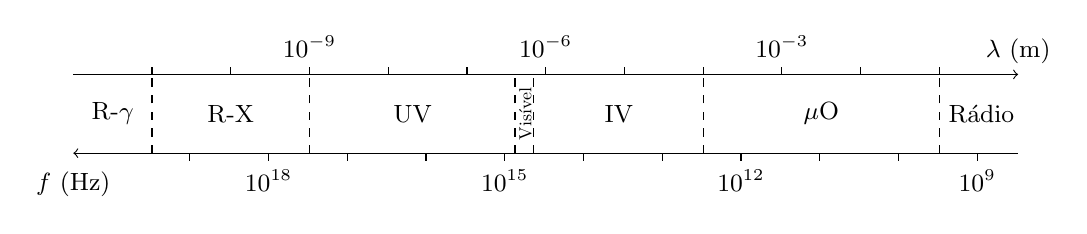
\begin{tikzpicture}
      \small
      \def\d{6}
      \draw [->] (-\d, 0.5) -- (\d,0.5) node [yshift=3mm]{$\lambda$ (m)};
      \draw [<-] (-\d,-0.5) node [yshift=-4mm]{$f$ (Hz)} -- (\d,-0.5);
      \foreach \i/\lbl [evaluate=\i as \x using -(\d-1) + 0.2*(\d-1)*(11+\i)] in
            {-11/ , -10/ , -9/$10^{-9}$,
              -8/ ,  -7/ , -6/$10^{-6}$,
              -5/ ,  -4/ , -3/$10^{-3}$,
              -2/ , -1/
            }{\draw (\x,0.5) -- +(0,0.1) node [above] {\lbl};}

      \node at(-5.5,0) {R-$\gamma$};
      \draw [dashed] (-5,-0.5) --+(0,1);
      \node at ( -4,0) {R-X};
      \draw [dashed] (-3,-0.5) --+(0,1);
      \node at ( -1.69,0) {UV};
      \draw [dashed] (-0.39,-0.5) --+(0,1);
      \draw [dashed] (-0.15,-0.5) --+(0,1);
      \node at (0.93,0) {IV};
      \draw [dashed] ( 2,-0.5) --+(0,1);
      \node at (3.5,0) {$\mu$O};
      \draw [dashed] ( 5,-0.5) --+(0,1);
      \node at (5,0) [right]{Rádio};
      \node at (-0.26,0) [rotate=90,scale=0.7] {Visível};

      \foreach \x/\f in { -4.52/ , -3.52/$10^{18}$, -2.52/ ,
                          -1.52/ , -0.52/$10^{15}$,  0.48/ ,
                           1.48/ ,  2.48/$10^{12}$,  3.48/ ,
                           4.48/ ,  5.48/$10^9$} {
        \draw (\x,-0.5) --+(0,-0.1) node [below]{\f};
      }
      
    \end{tikzpicture}
    \caption{O espectro eletromagnético.\label{fig:elmgspec}}\par
  }
\end{figure}
Como se pode verificar nesta figura, a parte do espectro eletromagnético a que
os nossos olhos são sensíveis, aquilo a que chamamos luz visível, é uma fatia
estreita de comprimentos de onda.

Dentro da gama visível, diferentes comprimentos produzem esstímulos visuais que
correspodem a diferentes sensações de cor. Considerando uma ordem crescente de
comprimentos de onda temos sucessivamente sensações visuais correspondentes às
cores violeta, azul, verde, amarelo, laranja e vermelho.



\section{Fotões}
Em 1900, o estudo da radiação térmica levou Plank a sugerir que as trocas de
energia entre a matéria e a radiação são inerentemente discretizadas, no sentido
em que quando um corpo emite ou absorve radiação, a energia envolvida no
processo é sempre um múltiplo inteiro de uma quantidade básica, chamada
\emph{quantum} de energia, proporcional à frequência da radiação emitida ou
absorvida. Em 1905, Einstein explicou esta discretização das trocas de energia
entre a matéria e a radiação, considerando que a própria radiação existia
apenas numa forma discretizada, como grãos ou partículas de luz com energia
proporcional à sua frequência. A hipótese corpuscular de Newton voltou assim a
emergir, mas agora numa forma híbrida, já que a teoria ondulatória, suportada
pelas equações de Maxwell, não foi abandonada.

As partículas de luz (ou seja, os fotões) têm aspetos particulares que as
distinguem dos corpos materiais mais vulgares. Em primeiro lugar, movem-se
sempre com velocidade igual à velocidade da luz no vazio,
$c=1/\sqrt{\epsilon_0\mu_0}$; depois, têm massa nula; e a sua energia cinética
depende apenas da frequência da radiação:
\begin{equation*}
    \varepsilon=hf.
\end{equation*}
A constante de proporcionalidade chama-se \emph{constante de Plank} e tem o
valor $h\simeq6,626\times10^{-3}$\,J\,s.

Numa abordagem corpuscular, consideramos que são os fotões os responsáveis pelo
transforte de energia num feixe de radiação. Nesse caso, eles devem ser em
quantidade apropriada para promover esse transporte. Assim, deve verificar-se
que a irradiância do feixe (energia transportada por unidade de tempo e de área)
deve ser igual à densidade de fluxo de fotões (fotões por unidade de tempo e de
área), multiplicada pela energia de cada fotão, ou seja, para radiação
monocromática,
\begin{equation}
    I=hfn,
\end{equation}
onde $n$ representa a densidade de fluxo de fotões.


\section*{Ondas eletromagnéticas --- Resumo}

